\documentclass[11pt,a4paper]{article}

\usepackage[T1]{fontenc}
\usepackage[utf8]{inputenc}
\usepackage{lmodern}
\usepackage[french]{babel}
\usepackage{amsmath,amssymb,amsthm}
\usepackage[margin=2.4cm]{geometry}
\usepackage{graphicx}
\usepackage{booktabs}
\usepackage{float}
\usepackage[font=small,labelfont=bf]{caption}
\usepackage{microtype}
\usepackage{xcolor}
\usepackage[colorlinks=true,linkcolor=violet,urlcolor=violet,citecolor=violet]{hyperref}

% Generated by experiments/run_all.py: do not edit by hand.

\newcommand{\tableEigen}{%
$\mathrm{CP}_1$ & 4{,}7059 & 4{,}7059 & 36{,}2\,\% & 36{,}2\,\% \\
$\mathrm{CP}_2$ & 2{,}4970 & 2{,}4970 & 19{,}2\,\% & 55{,}4\,\% \\
$\mathrm{CP}_3$ & 1{,}4461 & 1{,}4461 & 11{,}1\,\% & 66{,}5\,\% \\
$\mathrm{CP}_4$ & 0{,}9190 & 0{,}9190 & 7{,}1\,\% & 73{,}6\,\% \\
$\mathrm{CP}_5$ & 0{,}8532 & 0{,}8532 & 6{,}6\,\% & 80{,}2\,\% \\
$\mathrm{CP}_6$ & 0{,}6417 & 0{,}6417 & 4{,}9\,\% & 85{,}1\,\% \\
}
\newcommand{\varDiff}{3{,}1 \times 10^{-15}}
\newcommand{\expOne}{36{,}2}
\newcommand{\expTwo}{19{,}2}
\newcommand{\cumTwo}{55{,}4}
\newcommand{\cumFive}{80{,}2}
\newcommand{\nKaiser}{3}
\newcommand{\skDiff}{1{,}2 \times 10^{-14}}
\newcommand{\rawOne}{99{,}8}
\newcommand{\rawTop}{proline}
\newcommand{\nccAcc}{97{,}2}
\newcommand{\tableCorr}{%
\texttt{flavanoids} & $+0{,}92$ & $-0{,}01$ \\
\texttt{total\_phenols} & $+0{,}86$ & $+0{,}10$ \\
\texttt{od280\_od315} & $+0{,}82$ & $-0{,}26$ \\
\texttt{proanthocyanins} & $+0{,}68$ & $+0{,}06$ \\
\texttt{nonflavanoid\_phenols} & $-0{,}65$ & $+0{,}05$ \\
\texttt{hue} & $+0{,}64$ & $-0{,}44$ \\
\texttt{proline} & $+0{,}62$ & $+0{,}58$ \\
\texttt{malic\_acid} & $-0{,}53$ & $+0{,}36$ \\
\texttt{alcalinity\_of\_ash} & $-0{,}52$ & $-0{,}02$ \\
\texttt{alcohol} & $+0{,}31$ & $+0{,}76$ \\
\texttt{magnesium} & $+0{,}31$ & $+0{,}47$ \\
\texttt{color\_intensity} & $-0{,}19$ & $+0{,}84$ \\
\texttt{ash} & $+0{,}00$ & $+0{,}50$ \\
}
\newcommand{\tableStability}{%
$10^{-2}$ & $1{,}2 \times 10^{-13}$ & $1{,}7 \times 10^{-16}$ \\
$10^{-4}$ & $5{,}7 \times 10^{-9}$ & $0$ \\
$10^{-6}$ & $9{,}0 \times 10^{-7}$ & $0$ \\
$10^{-8}$ & $1{,}0 \times 10^{0}$ & $0$ \\
$10^{-10}$ & $1{,}0 \times 10^{0}$ & $0$ \\
}
\newcommand{\svdTime}{17{,}2}
\newcommand{\svErr}{7{,}6 \times 10^{-14}}
\newcommand{\tableCompression}{%
1 & 0{,}4\,\% & 0{,}4595 & 0{,}4595 & 12{,}1 \\
5 & 2{,}0\,\% & 0{,}2855 & 0{,}2855 & 16{,}3 \\
10 & 3{,}9\,\% & 0{,}2053 & 0{,}2053 & 19{,}2 \\
20 & 7{,}8\,\% & 0{,}1438 & 0{,}1438 & 22{,}3 \\
50 & 19{,}6\,\% & 0{,}0787 & 0{,}0787 & 27{,}6 \\
100 & 39{,}1\,\% & 0{,}0415 & 0{,}0415 & 33{,}1 \\
200 & 78{,}2\,\% & 0{,}0155 & 0{,}0155 & 41{,}7 \\
}
\newcommand{\eyGap}{3{,}5 \times 10^{-15}}
\newcommand{\psnrFifty}{27{,}6}
\newcommand{\errFifty}{7{,}9}
\newcommand{\storeFifty}{19{,}6}


\newtheorem{proposition}{Proposition}
\newtheorem{theoreme}{Théorème}
\theoremstyle{remark}
\newtheorem*{remarque}{Remarque}

\newcommand{\R}{\mathbb{R}}
\DeclareMathOperator{\rg}{rg}
\DeclareMathOperator{\tr}{tr}

\title{\textbf{Analyse en composantes principales\\ et décomposition en valeurs singulières}}
\author{Yassine Abderrezak Dache\\[2pt]\small Projet personnel \textendash{} Python (NumPy, Matplotlib)\\[1pt]\small\url{https://github.com/yassinedache/pca-svd-from-scratch}}
\date{\today}

\begin{document}
\maketitle

\begin{abstract}
On programme deux algorithmes de rotations de Jacobi, l'un pour diagonaliser une matrice symétrique et l'autre pour calculer la décomposition en valeurs singulières (SVD), sans faire appel aux routines de NumPy. Ils servent d'abord à réaliser l'analyse en composantes principales (ACP) du jeu de données \emph{Wine} par deux voies, la diagonalisation de la matrice de covariance puis la SVD de la matrice des données : les deux voies coïncident à $\varDiff$ près, et le premier plan factoriel sépare les trois cépages (\nccAcc\,\% de vins bien classés par une règle du centre le plus proche). On montre ensuite pourquoi la voie SVD est numériquement préférable. Enfin, on compresse une image $512 \times 512$ par approximation de rang faible et l'on vérifie le théorème d'Eckart\textendash Young : l'erreur mesurée coïncide avec la formule théorique à $\eyGap$ près.
\end{abstract}

\section{Rappels : diagonalisation et SVD}

\begin{theoreme}[Théorème spectral]
Toute matrice symétrique réelle $S \in \R^{p\times p}$ s'écrit $S = V \Lambda V^\top$ avec $V$ orthogonale et $\Lambda = \mathrm{diag}(\lambda_1 \ge \dots \ge \lambda_p)$.
\end{theoreme}

\begin{theoreme}[Décomposition en valeurs singulières]
Toute matrice $A \in \R^{m \times n}$ s'écrit $A = U \Sigma V^\top = \sum_{i=1}^{r} \sigma_i\, u_i v_i^\top$ avec $U$, $V$ à colonnes orthonormées, $\sigma_1 \ge \dots \ge \sigma_r > 0$ et $r = \rg A$.
\end{theoreme}

Les deux décompositions sont liées : $A^\top A = V \Sigma^2 V^\top$. Les valeurs singulières de $A$ sont donc les racines carrées des valeurs propres de $A^\top A$, et ses vecteurs singuliers à droite sont les vecteurs propres de $A^\top A$.

\subsection{Méthode de Jacobi pour une matrice symétrique}

Une rotation de Givens $J(p,q,\theta)$ agit seulement sur les lignes et colonnes $p$ et $q$. On choisit $\theta$ pour annuler le coefficient $s_{pq}$ de $J^\top S J$ :
\[
  \tan 2\theta = \frac{2 s_{pq}}{s_{qq} - s_{pp}} .
\]
Comme la norme de Frobenius est invariante par rotation, la masse hors diagonale $\mathrm{off}(S)^2 = \sum_{i\ne j} s_{ij}^2$ diminue exactement de $2 s_{pq}^2$ à chaque rotation. En balayant tous les couples $(p,q)$, $\mathrm{off}(S) \to 0$ (la convergence est même quadratique en fin de calcul), et le produit des rotations donne les vecteurs propres.

\subsection{SVD par la méthode de Jacobi « à un côté »}

Au lieu de diagonaliser $A^\top A$, on applique des rotations à droite de $A$ : pour un couple de colonnes $(a_p, a_q)$, on choisit la rotation qui les rend orthogonales. Cela revient à appliquer la méthode précédente à $A^\top A$, mais sans jamais former ce produit. Quand toutes les colonnes de $AV$ sont orthogonales, on a $AV = U\Sigma$ : les normes des colonnes sont les valeurs singulières. Pour rendre l'algorithme rapide en Python, on traite à chaque étape $n/2$ couples disjoints simultanément (ordre « round-robin ») avec des opérations vectorisées de NumPy. La SVD de l'image $512\times512$ prend ainsi $\svdTime$~s, et ses valeurs singulières diffèrent de celles de NumPy de $\svErr$ en relatif.

\section{Analyse en composantes principales}

\subsection{Deux façons de la calculer}

Soit $X \in \R^{n\times p}$ la matrice des données centrées (et réduites), une ligne par individu. L'ACP cherche les directions $v$ de variance maximale : la variance des projections $Xv$ vaut $v^\top C v$, avec $C = \frac{1}{n-1} X^\top X$ la matrice de covariance (ou de corrélation pour des données réduites).

\begin{proposition}
Le maximum de $v^\top C v$ sous la contrainte $\lVert v\rVert = 1$ vaut $\lambda_1$ et il est atteint pour le premier vecteur propre $v_1$ de $C$. Plus généralement, les axes principaux sont les vecteurs propres $v_1, \dots, v_p$ et la variance le long de $v_j$ est $\lambda_j$.
\end{proposition}

\begin{proof}
On décompose $v = \sum_j c_j v_j$ dans la base orthonormée des vecteurs propres. Alors $v^\top C v = \sum_j \lambda_j c_j^2 \le \lambda_1 \sum_j c_j^2 = \lambda_1$, avec égalité pour $v = v_1$. On obtient les axes suivants en répétant le raisonnement dans l'orthogonal des axes déjà trouvés.
\end{proof}

\begin{enumerate}
  \item \textbf{Voie covariance} : on forme $C$ puis on la diagonalise par la méthode de Jacobi.
  \item \textbf{Voie SVD} : on calcule $X = U\Sigma V^\top$. Comme $C = V \frac{\Sigma^2}{n-1} V^\top$, les axes principaux sont les colonnes de $V$, les variances sont $\lambda_j = \sigma_j^2/(n-1)$, et les coordonnées des individus sont $XV = U\Sigma$.
\end{enumerate}

\subsection{Application au jeu de données Wine}

Le jeu de données \emph{Wine} (UCI, Aeberhard et Forina) décrit 178 vins italiens issus de trois cépages par 13 mesures chimiques (alcool, acide malique, flavanoïdes, intensité de la couleur, proline, etc.). Les variables ont des unités et des ordres de grandeur très différents, on les réduit donc avant l'analyse. Sans cette réduction, la première composante expliquerait $\rawOne$\,\% de la variance et ne serait presque que la variable \texttt{\rawTop}, dont les valeurs sont de l'ordre de 1\,000.

\begin{table}[htbp]
\centering
\begin{tabular}{lcccc}
\toprule
Axe & $\lambda_j$ (covariance, Jacobi) & $\sigma_j^2/(n-1)$ (SVD) & Variance expliquée & Cumul \\
\midrule
\tableEigen
\bottomrule
\end{tabular}
\caption{Les deux voies donnent les mêmes valeurs à $\varDiff$ près (et la même chose que \texttt{scikit-learn}, à $\skDiff$ près). Pour des données réduites, $\sum_j \lambda_j = \tr C = 13$.}
\end{table}

Les deux premières composantes résument $\cumTwo$\,\% de l'information et les cinq premières $\cumFive$\,\%. Le critère de Kaiser (conserver les axes de valeur propre supérieure à 1, soit plus d'information qu'une variable initiale) retient $\nKaiser$ composantes.

\begin{figure}[htbp]
\centering
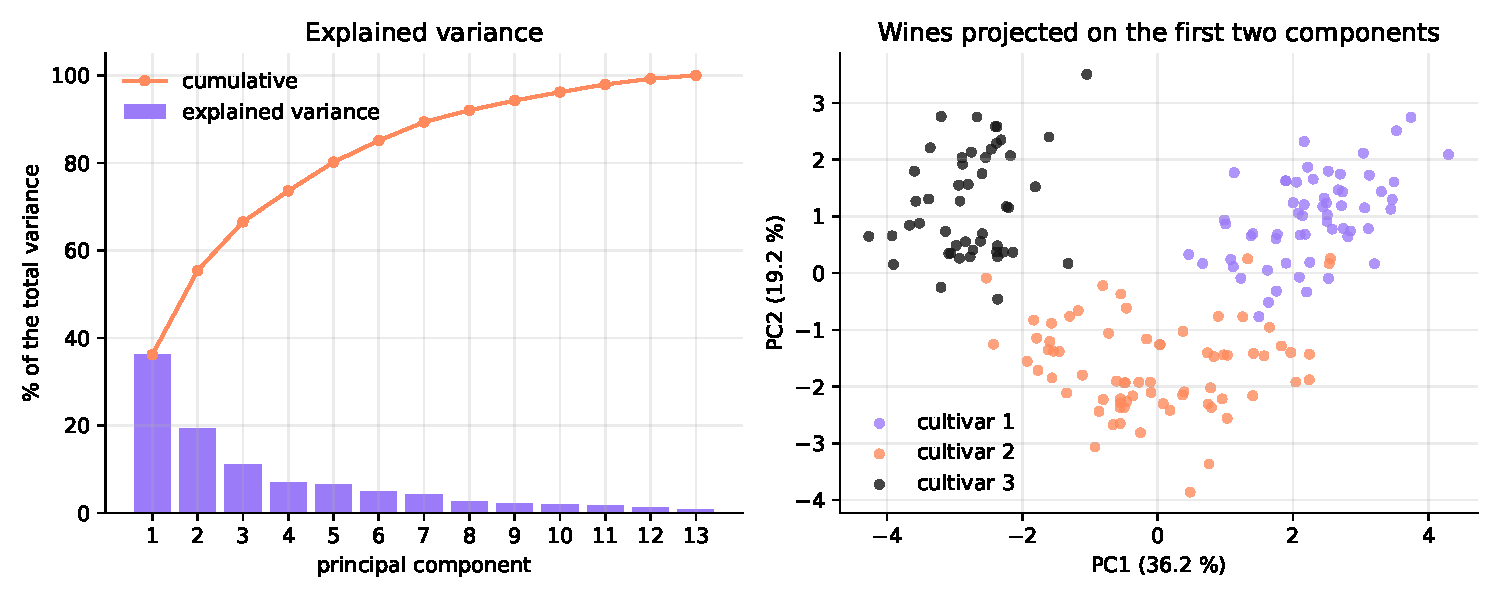
\includegraphics[width=\textwidth]{../figures/1_wine_pca.pdf}
\caption{Éboulis des valeurs propres et projection des 178 vins sur le premier plan factoriel.}
\end{figure}

\subsection{Interprétation}

Pour des données réduites, la corrélation entre la variable $j$ et la composante $k$ vaut $v_{jk}\sqrt{\lambda_k}$. Le cercle des corrélations permet de nommer les axes.

\begin{minipage}{0.47\textwidth}
\centering
\small
\begin{tabular}{lcc}
\toprule
Variable & $\mathrm{CP}_1$ & $\mathrm{CP}_2$ \\
\midrule
\tableCorr
\bottomrule
\end{tabular}
\end{minipage}\hfill
\begin{minipage}{0.5\textwidth}
\centering
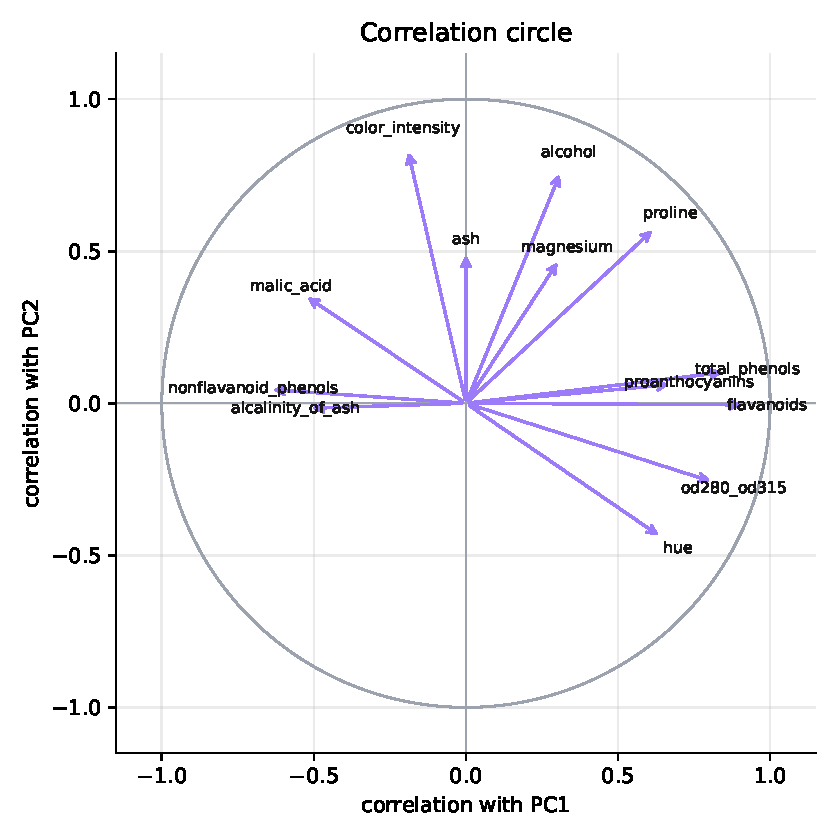
\includegraphics[width=\textwidth]{../figures/2_correlation_circle.pdf}
\end{minipage}

\medskip
La première composante oppose les vins riches en composés phénoliques (flavanoïdes, phénols totaux, rapport OD280/OD315) à ceux qui ont davantage de phénols non flavanoïdes et d'acide malique. La deuxième est portée par l'intensité de la couleur, le degré d'alcool et la proline. Dans ce plan, les trois cépages forment trois groupes distincts : le cépage 1 a des scores élevés sur les deux axes, le cépage 3 un score faible sur le premier, et le cépage 2 se situe en bas. Une règle simple, qui affecte chaque vin au cépage dont le centre est le plus proche dans ce plan (validée en laissant chaque vin de côté tour à tour), classe correctement $\nccAcc$\,\% des vins, alors que l'ACP n'a jamais utilisé l'étiquette des cépages.

\subsection{Pourquoi préférer la voie SVD}

Former $X^\top X$ élève le conditionnement au carré : une valeur singulière $\sigma$ devient la valeur propre $\sigma^2$, et si $\sigma^2$ est inférieure à $\varepsilon\,\sigma_1^2$ (avec $\varepsilon \approx 10^{-16}$ la précision machine), elle est noyée dans les erreurs d'arrondi. On le vérifie sur la matrice de Läuchli
\[
A = \begin{pmatrix} 1 & 1 & 1 \\ \epsilon & 0 & 0 \\ 0 & \epsilon & 0 \\ 0 & 0 & \epsilon \end{pmatrix},
\qquad
A^\top A = \begin{pmatrix} 1+\epsilon^2 & 1 & 1 \\ 1 & 1+\epsilon^2 & 1 \\ 1 & 1 & 1+\epsilon^2 \end{pmatrix},
\]
dont la plus petite valeur singulière vaut exactement $\epsilon$. Dès que $\epsilon^2 < \varepsilon$, le nombre $1+\epsilon^2$ est arrondi à $1$ et l'information est perdue.

\begin{table}[htbp]
\centering
\begin{tabular}{ccc}
\toprule
$\epsilon$ & Erreur relative (valeurs propres de $A^\top A$) & Erreur relative (SVD de $A$) \\
\midrule
\tableStability
\bottomrule
\end{tabular}
\caption{La voie covariance perd la moitié des chiffres significatifs puis tous ; la SVD reste exacte.}
\end{table}

\section{Compression d'images par approximation de rang faible}

\subsection{Le théorème d'Eckart\textendash Young}

Une image en niveaux de gris est une matrice $A \in \R^{m \times n}$. On l'approche par la somme tronquée $A_k = \sum_{i=1}^{k} \sigma_i u_i v_i^\top$, dont le stockage demande $k(m+n+1)$ nombres au lieu de $mn$.

\begin{theoreme}[Eckart\textendash Young\textendash Mirsky]
Pour toute matrice $B$ de rang au plus $k$,
\[
  \lVert A - B\rVert_F \ \ge\ \lVert A - A_k\rVert_F = \Big(\sum_{i>k} \sigma_i^2\Big)^{1/2}
  \quad\text{et}\quad
  \lVert A - B\rVert_2 \ \ge\ \lVert A - A_k\rVert_2 = \sigma_{k+1} .
\]
\end{theoreme}

\begin{proof}[Idée de la preuve (norme spectrale)]
Si $\rg B \le k$, le noyau de $B$ est de dimension au moins $n-k$ ; il rencontre donc le sous-espace de dimension $k+1$ engendré par $v_1,\dots,v_{k+1}$. On y choisit un vecteur unitaire $x = \sum_{i\le k+1} c_i v_i$ : alors $\lVert (A-B)x\rVert = \lVert Ax\rVert = \big(\sum_{i \le k+1} \sigma_i^2 c_i^2\big)^{1/2} \ge \sigma_{k+1}$. Enfin, $A - A_k = \sum_{i>k}\sigma_i u_i v_i^\top$ a pour plus grande valeur singulière $\sigma_{k+1}$, et pour norme de Frobenius $\big(\sum_{i>k}\sigma_i^2\big)^{1/2}$ par orthonormalité.
\end{proof}

\subsection{Expérience}

On utilise une photographie $512 \times 512$ du domaine public (NASA), convertie en niveaux de gris. Le tableau compare l'erreur relative mesurée $\lVert A - A_k\rVert_F / \lVert A\rVert_F$ à la formule du théorème, calculée à partir des seules valeurs singulières. Le PSNR (rapport signal sur bruit de crête) est la mesure de qualité usuelle en traitement d'images : au-delà d'environ 30~dB, la différence devient difficile à voir.

\begin{table}[htbp]
\centering
\begin{tabular}{ccccc}
\toprule
Rang $k$ & Données stockées & Erreur mesurée & Formule d'Eckart\textendash Young & PSNR (dB) \\
\midrule
\tableCompression
\bottomrule
\end{tabular}
\caption{L'écart maximal entre erreur mesurée et erreur théorique est de $\eyGap$. On a aussi vérifié que $\lVert A - A_k\rVert_2 = \sigma_{k+1}$ pour chaque $k$.}
\end{table}

\begin{figure}[htbp]
\centering
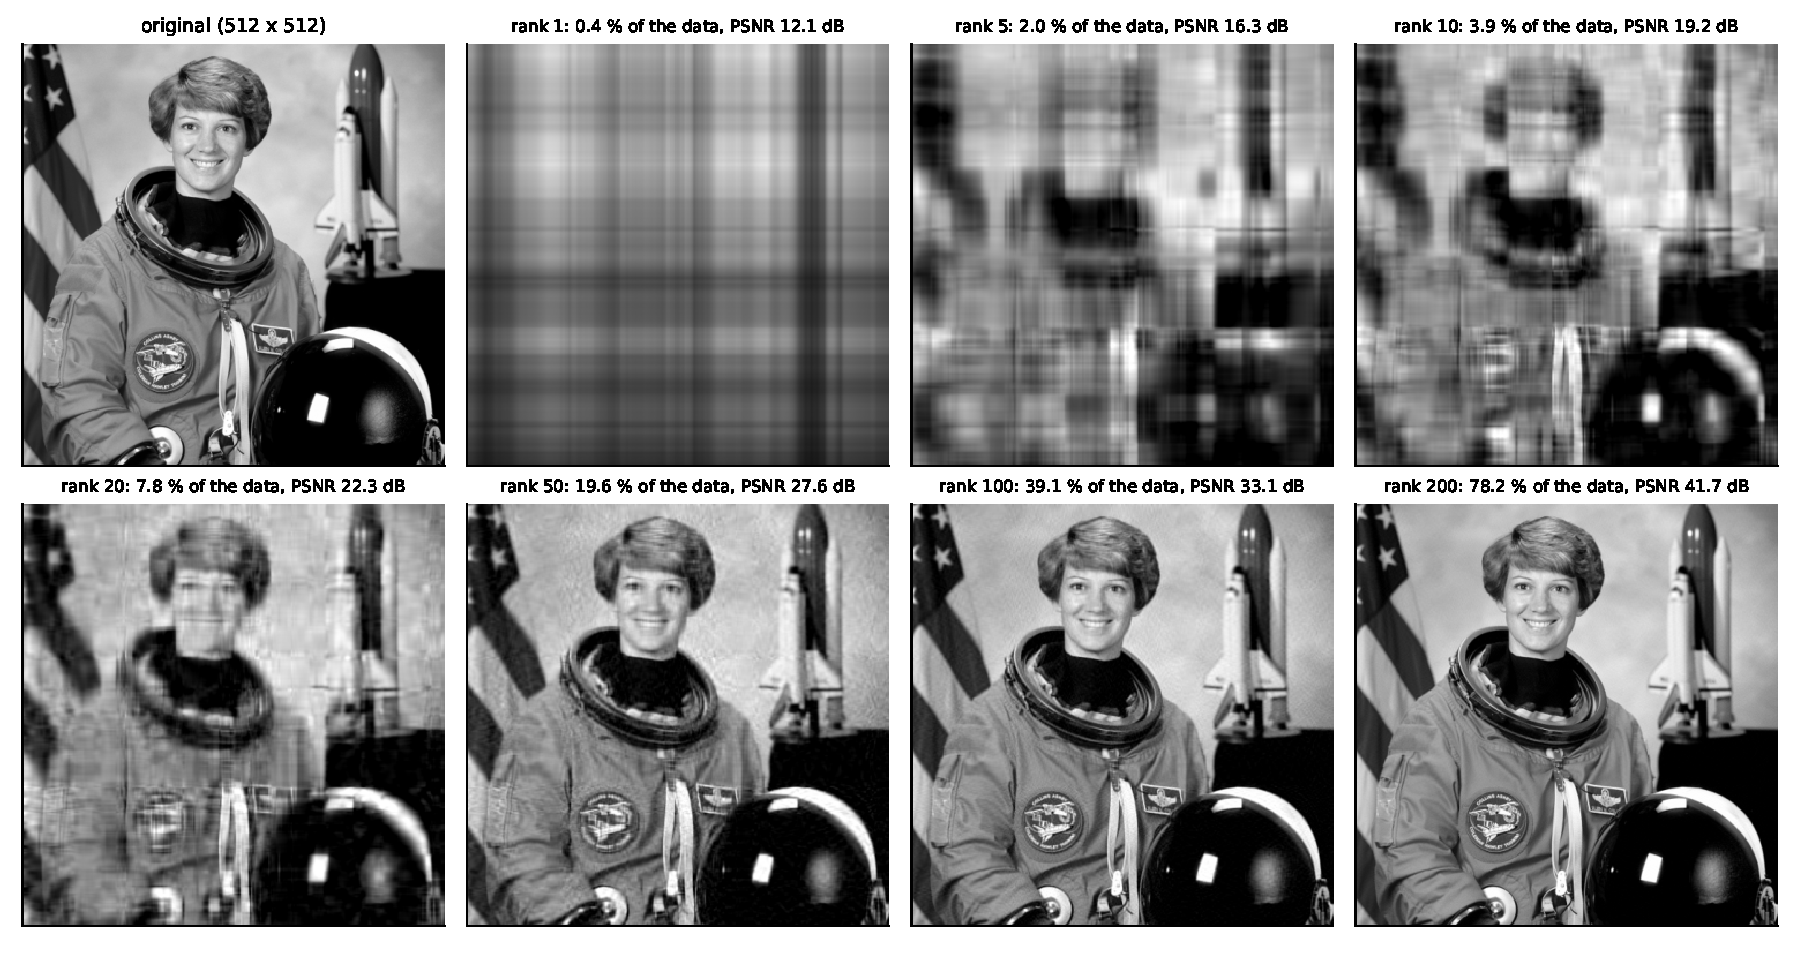
\includegraphics[width=\textwidth]{../figures/5_compression.pdf}
\caption{Reconstructions de rang croissant. Les premières composantes ne contiennent que la structure grossière de l'image (des motifs « en croix », car chaque terme $u_i v_i^\top$ est un produit d'une colonne par une ligne) ; les détails apparaissent progressivement.}
\end{figure}

Avec $k = 50$, on ne stocke que $\storeFifty$\,\% des nombres de l'image pour une erreur relative de $\errFifty$\,\% et un PSNR de $\psnrFifty$~dB.

\begin{figure}[htbp]
\centering
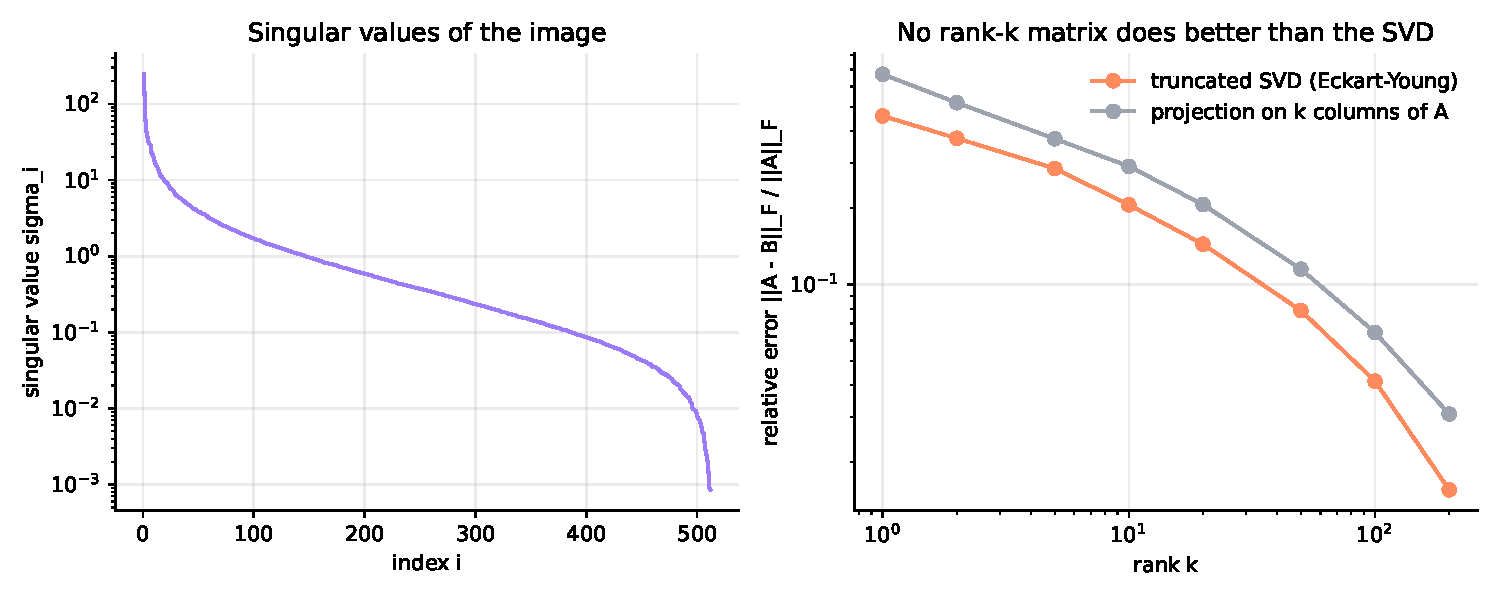
\includegraphics[width=\textwidth]{../figures/4_singular_values.pdf}
\caption{À gauche, la décroissance des valeurs singulières : quelques-unes concentrent l'essentiel de l'énergie de l'image, ce qui rend la compression efficace. À droite, l'optimalité de la SVD : une autre approximation de rang $k$ (projection sur $k$ colonnes de l'image) fait toujours moins bien.}
\end{figure}

\begin{figure}[htbp]
\centering
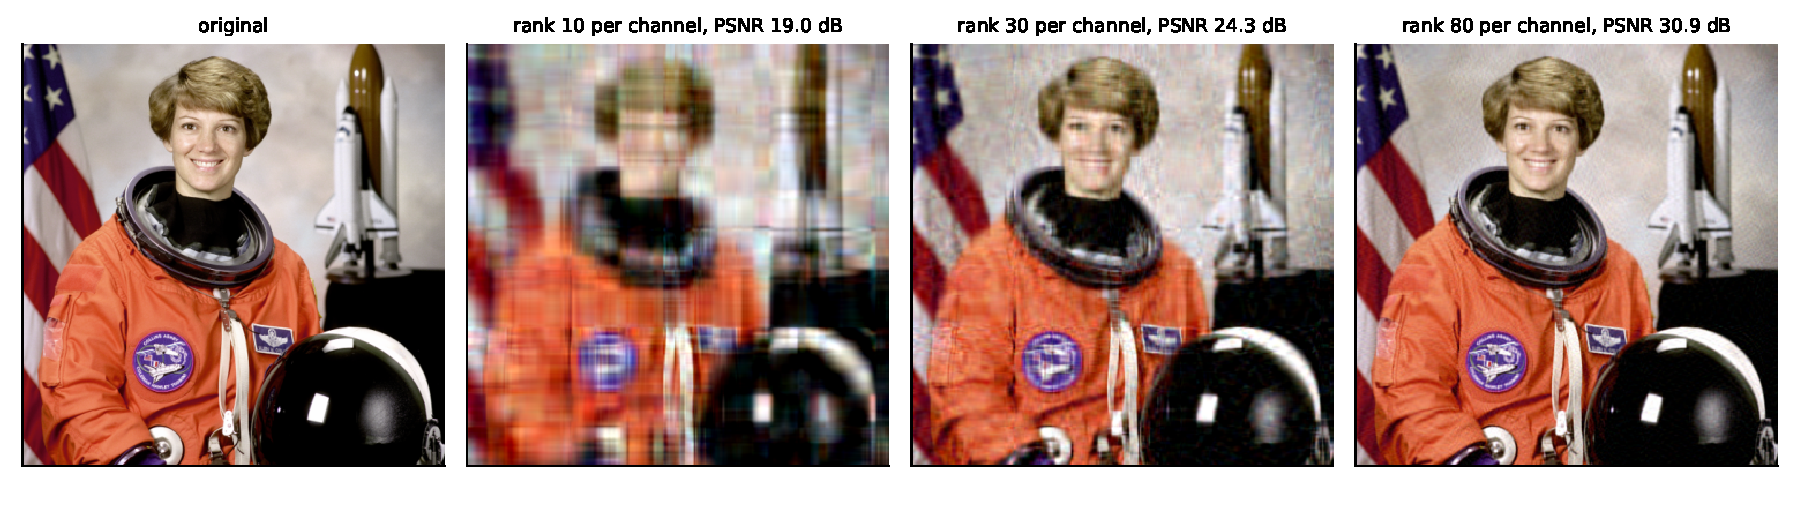
\includegraphics[width=\textwidth]{../figures/6_compression_color.pdf}
\caption{Pour une image en couleurs, on applique la même méthode à chacun des trois canaux rouge, vert et bleu.}
\end{figure}

\begin{remarque}
Cette compression reste théorique : les formats comme JPEG font beaucoup mieux, car ils utilisent une base fixe (cosinus) adaptée à l'œil et un codage entropique. L'intérêt de l'expérience est de rendre visible le théorème d'Eckart\textendash Young, qui est aussi le fondement de l'ACP : les $k$ premières composantes principales donnent la meilleure approximation de rang $k$ du nuage de points centré.
\end{remarque}

\section{Conclusion}

La même décomposition, la SVD, sert à deux usages : réduire la dimension d'un jeu de données en conservant le plus de variance possible (ACP), et approcher une matrice par une matrice de rang faible avec une erreur minimale et connue à l'avance (Eckart\textendash Young). Les expériences confirment la théorie avec une précision proche de la précision machine, et montrent qu'il vaut mieux calculer la SVD de $X$ que diagonaliser $X^\top X$. Prolongements possibles : les méthodes de SVD tronquée par itération (puissance itérée, Lanczos) ou randomisées, adaptées aux très grandes matrices, et l'ACP à noyau pour les structures non linéaires.

\appendix
\section{Reproduire les résultats}

Toutes les valeurs numériques de ce document sont générées par le code :
\begin{verbatim}
pip install -r requirements.txt
python experiments/run_all.py     # figures, results.md et report/generated.tex
pytest                            # 16 tests
cd report && pdflatex rapport.tex
\end{verbatim}

\end{document}
